\chapter{Planificación}\label{cap:planificación}

\section{Estructura de descomposición del trabajo}

Para el desarrollo del proyecto se seguirá la metodología SCRUM por su aplicabilidad al proyecto, ya que al contar con un cliente real que debe validar cada parte del proyecto y del que se deben obtener los requisitos e información técnica, creo que es la metodología más útil para seguir por la facilidad de crear entregables que presentar al cliente y obtener la validación antes de continuar con nuevas funcionalidades.

A continuación, desglosaré la EDT del proyecto y luego la EDT específica de cada Sprint para que sea más fácil de seguir la planificación.

\subsection{EDT del proyecto}\label{cap:Planificación}

\begin{enumerate}
    \item Presentación del proyecto
    \item Análisis del conjunto del proyecto
    \item Elicitación general del proyecto
    \item Aceptación del alcance del proyecto
    \item Ciclo de Sprints
    \item Despliegue del proyecto
    \item Formación de usuarios
    \item Cierre del proyecto
\end{enumerate}

\subsection{EDT de cada Sprint}

\begin{enumerate}
    \item Reunión definición de objetivos
    \item Análisis
    \item Elicitación de requisitos
    \item Diseño
    \item Codificación
    \item Pruebas
    \item Validación con el cliente
    \item Reunión de fin de Sprint
\end{enumerate}

\section{Estimación temporal}

La duración de los Sprints es de 15 días y la dedicación diaria es de 3 horas. En un principio la estimación temporal del proyecto era de 5 días para las 4 primeras fases, 6 sprints en el ciclo de sprints y 5 días para el despliegue, formación de usuarios y cierre del proyecto.

Durante el último sprint se decidió un par de funcionalidades extras, lo que supuso añadir 1 sprint reducido, de 7 días, al ciclo de sprints, lo que hizo aumentar la duración total de 100 a 107 días.

Por lo tanto, la estimación inicial era realizar el proyecto en 300 horas de trabajo, pero debido a los retrasos y a los imprevistos conllevaron una nueva previsión de 321 horas. Esto supone una desviación temporal del 7\% respecto a la estimación inicial.

\bigskip

\begin{center}
    \begin{tabulary}{0.8\textwidth}{|L|L|L|L|}
        \hline
            \textbf{Tarea} & \textbf{Estimación inicial (Horas)} & \textbf{Estimación Final (Horas)} \\
            \hline
            Búsqueda de documentación & 30 & 35 \\
            \hline
            Introducción y planificación & 10 & 10 \\
            \hline
            Elicitación de requisitos & 30 & 30 \\
            \hline
            Análisis de requisitos & 10 & 10 \\
            \hline
            Diseño del sistema & 10 & 10 \\
            \hline
            Implementación & 160 & 170 \\
            \hline
            Pruebas & 20 & 25 \\
            \hline
            \textbf{Total} & \textbf{300} & \textbf{321} \\
            \hline
    \end{tabulary}
\end{center}

\bigskip

A continuación, podremos observar de una forma más visual los tiempos ejercidos para cada tarea mediante un diagrama de Gantt.

\textbf{Nota: los periodos deben ser tratados como una aproximación de 10 horas.}

\bigskip

\begin{figure}[H]
    \centering
    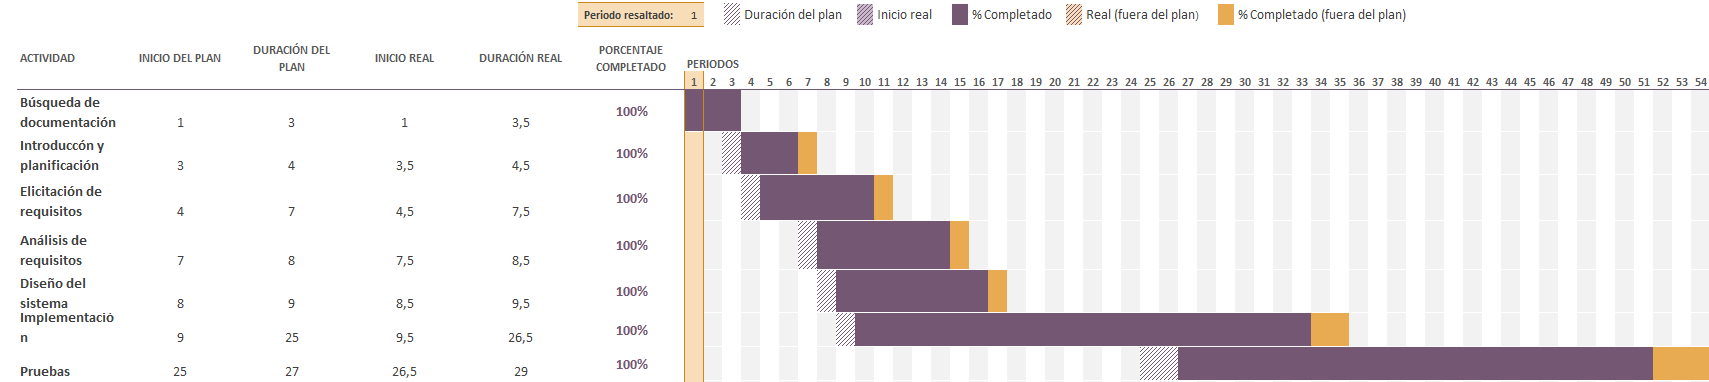
\includegraphics[width=1\linewidth]{fig/gantt.png}
    \caption{Diagrama de Gantt}
    \label{fig:gantt}
\end{figure}

\section{Estimación de coste del proyecto}

Para poder estimar el coste me basaré exclusivamente en las horas requeridas para el desarrollo y análisis del problema, así como las reuniones y trato con el cliente. En el apartado del coste material solo habría que mencionar el coste del ordenador usado, pero debido a que la aplicación está enfocada a dispositivos móviles de uso doméstico no veo relevante indicar las especificaciones del ordenador usado para el desarrollo, ya que un ordenador doméstico de gama baja hubiese sido de la misma utilidad.

Respecto a la estimación de costes del personal, y como he mencionado anteriormente en el documento, el proyecto constó de 270 horas asumidas por el alumno encargado de este TFG como desarrollador.

Obteniendo la información del sueldo medio de desarrollador Android, obtenemos que el sueldo medio percibido por año en España es de 31.994 €. Si realizamos los cálculos con las horas empleadas en este proyecto, obtenemos que el coste final del personal sería de \textbf{16,7 €/h * 270h = 4509 €}.

\newpage

\newpage